\documentclass{report}
\usepackage{graphicx}

\usepackage{amsmath}
\DeclareMathOperator*{\argmax}{argmax}

\usepackage{hyperref}
\hypersetup{
    colorlinks=true,
    linkcolor=blue,
    filecolor=magenta,      
    urlcolor=cyan,
}

\begin{document}

\title{Banana World Project Report}
\author{Denis Sergeev}


\section*{Problem definition}

The goal of the project was to create a RL Agent which is able to learn from scratch by interacting with the Tennis environment for a series of episodes. The episode is divided into discrete time intervals. After each time interval the the agent receives the environment state. The agent is able to perform some actions after each time interval which may change the environment state.

\subsection*{Environment description}

In this environment, two agents control rackets to bounce a ball over a net. If an agent hits the
ball over the net, it receives a reward of \(+0.1\). If an agent lets a ball hit the ground or hits the ball out of bounds, it receives a reward of -0.01. Thus, the goal of each agent is to keep the ball in play.

The observation space consists of 8 variables corresponding to the position and velocity of the
ball and racket. Each agent receives its own, local observation. Two continuous actions are available, corresponding to movement toward (or away from) the net, and jumping.

The task is episodic, and in order to solve the environment, the agents must get an average score of \(+0.5\) (over 100 consecutive episodes, after taking the maximum over both agents). Specifically,

\begin{itemize}
\item After each episode, we add up the rewards that each agent received (without discounting), to get a score
for each agent. This yields 2 (potentially different) scores. We then take the maximum of these 2 scores.
\item This yields a single score for each episode.
\end{itemize}


\section*{Solution}
\subsection*{Deep Deterministic Policy Gradient Algorithm}
\subsubsection*{Network}

Since the environment is not competitive but collaborative and both agents have same task and observe mirrored state of the environment, I decided to use simple DDPG algorithm and train both agents on single pair of actor/critic network, instead of training them separately.

The DDPG algorithm uses two neural networks, an actor and a critic. Each one has two copies, a local and a target one. The Actor is trained to give the best possible action, given the current state of the environment. \(s => a\). The Critic is trained to give an estimate of the reward that'd be obtained if an action A is applied at the state \(s\). \((s, a) => V\) Local networks are trained to get the "labels" given by the target.

Both networks consist of fully connected units with batch normalization and ReLu activation. The input to the actor network is the environment state, which goes through 3 fully connected layers. The final activation function is \(tanh\), since the action value should be in-between \(-1\) and \(1\).

The input to the critic is the environment state, which goes through the first fully connected layer. After batch normalization and ReLu activation it is concatenated with the action tensor and goes through the remaining 2 layers.

\subsection*{Training}
\subsubsection*{Loss function and optimizing method}

DDGP algorithm uses following loss function for critic network \ref{critic-loss}:
\begin{equation} \label{critic-loss}
L \equiv (R_t + \gamma Q(S_{t+1}, a_{t+1}; \theta'_t) - Q(S_t, a_t; \theta_t))^{2}
\end{equation}

Where \(Q(S_t, a_t; \theta_t)\) is output (value of action) of the critic network with internal parameters \(\theta_t\) given input \(S_t\) and \(a_t\). \(a_{t+1}\) is obtained from \(\pi(S_t; \eta'_t)\) (target actor) prediction with internal parameters \(\eta'_t\).

Actor loss function is following \ref{actor-loss}:
\begin{equation} \label{actor-loss}
L \equiv -(Q(S_t, \pi(S_t; \eta_t); \theta_t))
\end{equation}

Both loss functions used 2 sets of network parameters: target \(\theta'_t\), \(\eta'_t\) and local \(\theta_t\), \(\eta_t\). Target network parameters are updating through soft update \(\theta'_t = (1 - \tau) \theta'_t + \tau \theta_t\).
As optimizing method for both networks I used Adam with learning rate \(\alpha\).

\subsubsection*{Experience replay}
The input for training did not come directly from episodes. Instead I used experience replay technique (see \href{https://storage.googleapis.com/deepmind-media/dqn/DQNNaturePaper.pdf}{Human-level control through deep reinforcement learning}).
Also I have implemented \href{https://arxiv.org/pdf/1511.05952.pdf}{prioritized experience replay}. But I did not notice improvement in training while using it instead of simple replay.

\subsubsection*{Exploratory noise}
In order to make the agent explore the environment DDPG algorithm adds noise in it actions during training. I used \href{https://en.wikipedia.org/wiki/Ornstein-Uhlenbeck_process}{Ornstein–Uhlenbeck process} for this purpose.


\section*{Results}

I came up using following training hyper parameters:
\begin{itemize}
	\item Buffer size: 10e6
	\item Batch size: 1024
	\item \(\gamma\): 0.9
	\item \(\tau\): 0.001
	\item \(\alpha_{actor}\): 0.0001
	\item \(\alpha_{critic}\): 0.001
\end{itemize}
They were used across all training experiments below.



\subsection*{Training DDPG 64x32 64x32}

DDPG actor: 64x32, critic 64x(32+31).

Episode 100.	Average Score: 0.01.	Time elapsed: 1:04.

Episode 200.	Average Score: 0.01.	Time elapsed: 2:21.

Episode 300.	Average Score: 0.00.	Time elapsed: 3:35.

Episode 400.	Average Score: 0.02.	Time elapsed: 5:01.

Episode 500.	Average Score: 0.03.	Time elapsed: 6:36.

Episode 600.	Average Score: 0.05.	Time elapsed: 8:34.

Episode 700.	Average Score: 0.06.	Time elapsed: 10:39.

Episode 800.	Average Score: 0.04.	Time elapsed: 12:38.

Episode 900.	Average Score: 0.06.	Time elapsed: 14:56.

Episode 1000.	Average Score: 0.11.	Time elapsed: 18:18.

Episode 1100.	Average Score: 0.09.	Time elapsed: 20:58.

Episode 1200.	Average Score: 0.09.	Time elapsed: 23:42.

Episode 1300.	Average Score: 0.11.	Time elapsed: 26:57.

Episode 1400.	Average Score: 0.10.	Time elapsed: 29:56.

Episode 1500.	Average Score: 0.11.	Time elapsed: 33:29.

Episode 1600.	Average Score: 0.30.	Time elapsed: 43:18.

Episode 1700.	Average Score: 0.40.	Time elapsed: 56:31.

Episode 1800.	Average Score: 0.47.	Time elapsed: 72:25.

Environment solved in 1722 episodes!	Average Score: 0.50.	Time elapsed: 76:52. See \ref{fig:DDPG_64x32}.

\begin{figure}
	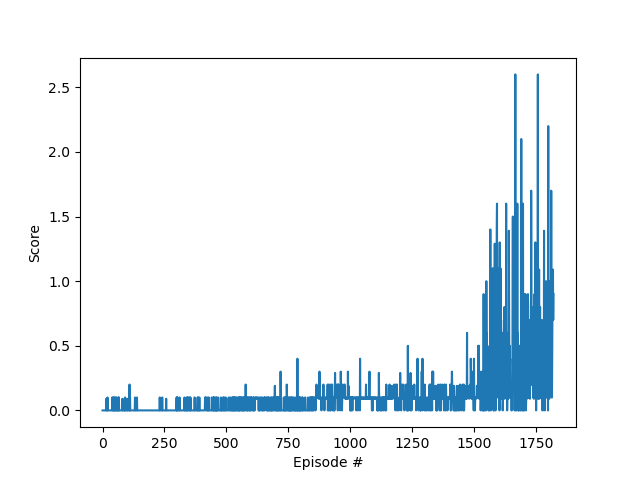
\includegraphics[width=0.9\linewidth]{res/ddpg_64x32/score.png}
	\caption{DDPG 64x32: Rewards per episode}
	\label{fig:DDPG_64x32}
\end{figure}



\subsection*{Training DDPG 64x32 64x32 with prioritized replay}

DDPG actor: 64x32, critic 64x(32+31).

Episode 100.	Average Score: 0.02.	Time elapsed: 1:05.

Episode 200.	Average Score: 0.02.	Time elapsed: 2:33.

Episode 300.	Average Score: 0.02.	Time elapsed: 3:59.

Episode 400.	Average Score: 0.02.	Time elapsed: 5:24.

Episode 500.	Average Score: 0.04.	Time elapsed: 7:10.

Episode 600.	Average Score: 0.05.	Time elapsed: 9:21.

Episode 700.	Average Score: 0.09.	Time elapsed: 12:26.

Episode 800.	Average Score: 0.11.	Time elapsed: 15:57.

Episode 900.	Average Score: 0.11.	Time elapsed: 19:52.

Episode 1000.	Average Score: 0.17.	Time elapsed: 25:28.

Episode 1100.	Average Score: 0.19.	Time elapsed: 31:33.

Episode 1200.	Average Score: 0.22.	Time elapsed: 39:04.

Episode 1300.	Average Score: 0.32.	Time elapsed: 50:28.

Episode 1400.	Average Score: 0.29.	Time elapsed: 60:57.

Episode 1500.	Average Score: 0.25.	Time elapsed: 69:48.

Episode 1600.	Average Score: 0.19.	Time elapsed: 77:12.

Episode 1700.	Average Score: 0.21.	Time elapsed: 84:53.

Episode 1800.	Average Score: 0.30.	Time elapsed: 96:14.

Episode 1900.	Average Score: 0.27.	Time elapsed: 106:36.

Episode 2000.	Average Score: 0.34.	Time elapsed: 119:37.

Episode 2100.	Average Score: 0.26.	Time elapsed: 130:05.

Episode 2200.	Average Score: 0.32.	Time elapsed: 143:45.

Episode 2300.	Average Score: 0.28.	Time elapsed: 155:33.

Episode 2400.	Average Score: 0.35.	Time elapsed: 170:28.

Episode 2500.	Average Score: 0.33.	Time elapsed: 185:15.

Episode 2600.	Average Score: 0.32.	Time elapsed: 199:51.

Episode 2700.	Average Score: 0.39.	Time elapsed: 218:28.

Episode 2800.	Average Score: 0.35.	Time elapsed: 235:13.

Episode 2900.	Average Score: 0.36.	Time elapsed: 252:47.

Environment solved in 2885 episodes!	Average Score: 0.51.	Time elapsed: 275:05 See \ref{fig:DDPG_64x32_pri}.

\begin{figure}
	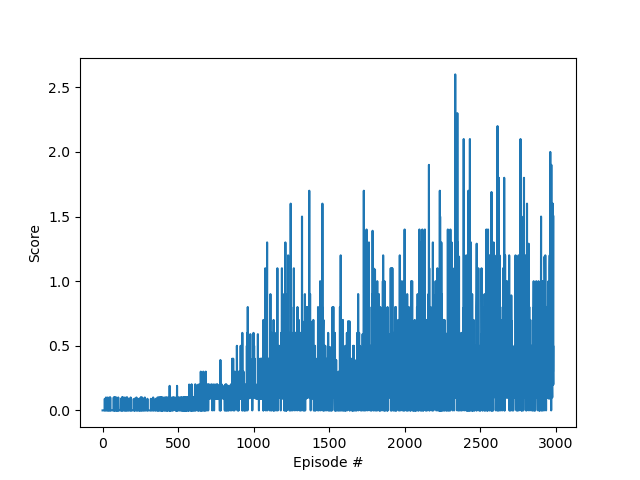
\includegraphics[width=0.9\linewidth]{res/ddpg_64x32_2/score.png}
	\caption{DDPG 64x32 with prioritized replay: Rewards per episode}
	\label{fig:DDPG_64x32_pri}
\end{figure}


\section*{Areas of improvement}

One possible improvement could be implementing \href{https://arxiv.org/pdf/1707.06347.pdf}{PPO algorithm} instead of DDPG. It should be working more stably.

Another one improvement could be staying with DDPG and play with hyperparameters to achieve faster training.


\section*{Conclusion}

From the above results we can summarize, that the Tennis environment is not a real multi-agent environment and it is possible to solve it just using regular DDPG algorithm. However the training process is very unstable. We can see this on the scores plot \ref{fig:DDPG_64x32}.

For a competitive and non-symmetric environment I would implement \href{https://arxiv.org/pdf/1706.02275.pdf}{MADDPG algorithm}.

\end{document}
